\documentclass[10pt,a4paper,openany]{beamer}
\usepackage[utf8]{vietnam}
\usepackage{lmodern}
\usetheme{AnnArbor}
\usecolortheme{dolphin}
\usepackage{tikz}
\usepackage{smartdiagram}
\usepackage{hyperref}

\AtBeginSection[]
{
	\begin{frame}<beamer>
		\frametitle{Outline}
		\tableofcontents[currentsection]
		
		\raggedright\tiny\textsuperscript{} Source code: \emph{\color{blue}\href{https://gitlab.ftech.ai/nlp/research/exercises-recommendation}{https://gitlab.ftech.ai/nlp/research/exercises-recommendation}}
		
		\raggedright\tiny\textsuperscript{} Documents: \emph{\color{blue}\href{https://docs.google.com/document/d/1J11qjjtteFJDZnR8BaAcA\_ny6hT3wbt-ceO8G7hdKsk}{https://docs.google.com/document/d/1J11qjjtteFJDZnR8BaAcA\_ny6hT3wbt-ceO8G7hdKsk}}
	\end{frame}
}

\author[phucpx]{}
\title{Exercises Recommendation System in AL \\ A Primitive Results}
\institute[]{}
\date{Ha Noi, Apr 28, 2021}
%
%
%
%
\newcommand{\argmax}{\arg\!\max}
%\subject{}
\tikzstyle{startstop} = [rectangle, rounded corners, minimum width=1.5cm, minimum height=0.6cm,text centered, draw=black, fill=red!30]
\tikzstyle{process} = [rectangle, minimum width=1.5cm, minimum height=0.6cm, text centered, draw=black, text width=2cm, fill=orange!30]
\tikzstyle{arrow} = [thick,->,>=stealth]

\setbeamertemplate{caption}[numbered] 
\begin{document}
	\listoffigures

	\begin{frame}
		\titlepage
	\end{frame}
	
	\section{Introduction}
	\begin{frame}{Introduction}
		\begin{itemize}
			\item Recommendation module is an important module in Adaptive learning systems.
			\item In order to consolidate the learning effect of students at certain stages, corresponding exercises are often provided to them appropriately. 
			\item It’s a challenge to recommend exercises with suitable difficulty levels for students as they have different learning status; variety of types; exercises bank is very large; knowledge concepts contained therein meet the requirements of the learning progress. 
		\end{itemize}
	\end{frame}
	
	
	\section{Approaches}
	\begin{frame}{Some approaches}
		\begin{itemize}
			\item Content-based Filtering (CBF) \footnote{\href{https://link.springer.com/chapter/10.1007\%2F978\-3\-540\-72079\-9\_10}{\text{\color{blue} Michael J. Pazzani, Daniel Billsus}, "Content-based Filtering" \emph{\href{https://link.springer.com/chapter/10.1007\%2F978\-3\-540\-72079\-9\_10}{\color{blue} In: https://link.springer.com/chapter/10.1007\%2F978\-3\-540\-72079\-9\_10}}}}
			
			\item Collaborative Filtering (CF) \footnote{\text{\color{blue} G. Linden}, "Amazon.com recommendations: item-to-item collaborative filtering" \emph{\color{blue} In: DOI: 10.1109/MIC.2003.1167344.}}  
			
			\item Hybrid Filtering based on similar - good learner's recommendation \footnote{\text{\color{blue} Dade Nurjanah}, "Good and Similar Learners' Recommendation  in Adaptive Learning Systems" \emph{\color{blue} In: Conference: 8th International Conference on Computer Supported Education. DOI: 10.5220/0005864304340440.}}
			
			\item Knowledge Concept Prediction - Exercises Recommendation (KCP-ER) \footnote{\text{\color{blue} ZhengyangWu}, "Exercise recommendation based on knowledge concept prediction" \emph{\color{blue} In: https://doi.org/10.1016/j.knosys.2020.106481.}}
		\end{itemize}
	\end{frame}
	
	\begin{frame}{Some approaches}
		\begin{itemize}
			\item Base on Knowledge Concept Prediction - Exercises Recommendation (KCP-ER)
			
			\item Pros and Cons:
				\begin{itemize}
					\item This method takes advantage of the output of Knowledge Tracing module, provides an efficient modeling method of measuring the performance of each learner -> more effective recommendation ;
					\item Allows configure the recommended exercises based on the desired difficulty level of the learner; or to diversify the difficulty level;
					\item There are many complicated modules: KCCP, KCMP, Filter layers
					\item Modules (KCCP, KCMP) using the DL model need enough data to train the model, leading to a cold-start problem.
				\end{itemize}
		\end{itemize}
	\end{frame}
	
	\section{Proposed approach}
	\begin{frame}{The proposed approach}
		\begin{figure}[htbp]
			\centerline{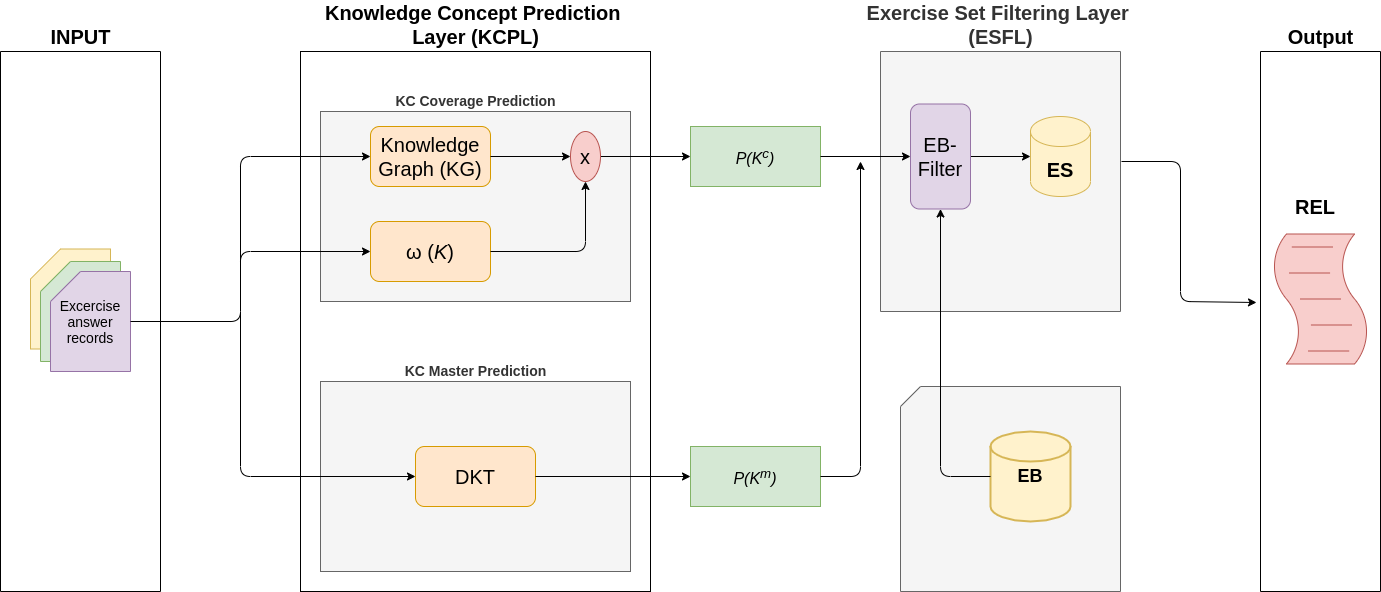
\includegraphics[scale=0.25]{charts/kcp_er.png}}
			\label{fig_motivation3}
			\caption{Pipeline the proposed System}
		\end{figure}
	\end{frame}	
	
	\begin{frame}{KCCP module}
		\begin{figure}[htbp]
			\centerline{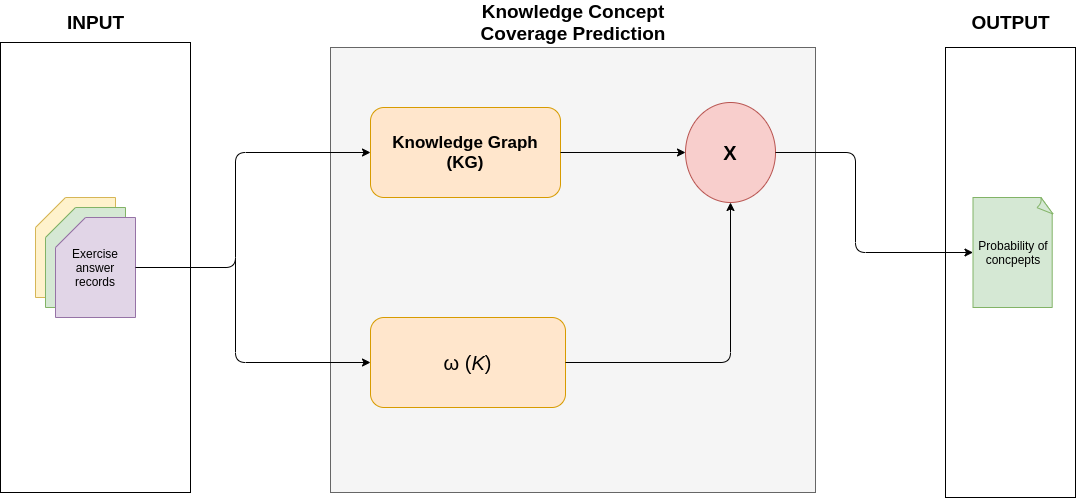
\includegraphics[scale=0.3]{charts/kgcp.png}}
			\label{fig_motivation3}
			\caption{Knowledge concept coverage prediction (KCCP) module}
		\end{figure}
	\end{frame}
	
	\begin{frame}{KT module}
		\begin{figure}[htbp]
			\centerline{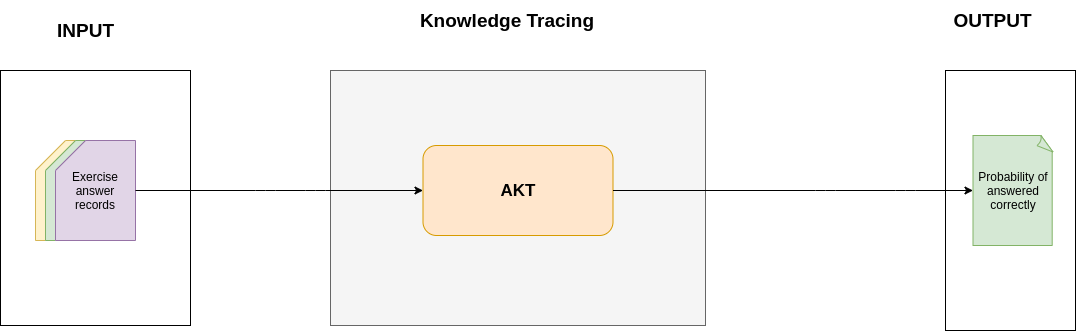
\includegraphics[scale=0.3]{charts/kt.png}}
			\label{fig_motivation3}
			\caption{Knowledge Tracing (KT) module}
		\end{figure}
	\end{frame}	
	
	\begin{frame}{Filter layer}
		\begin{figure}[htbp]
			\centerline{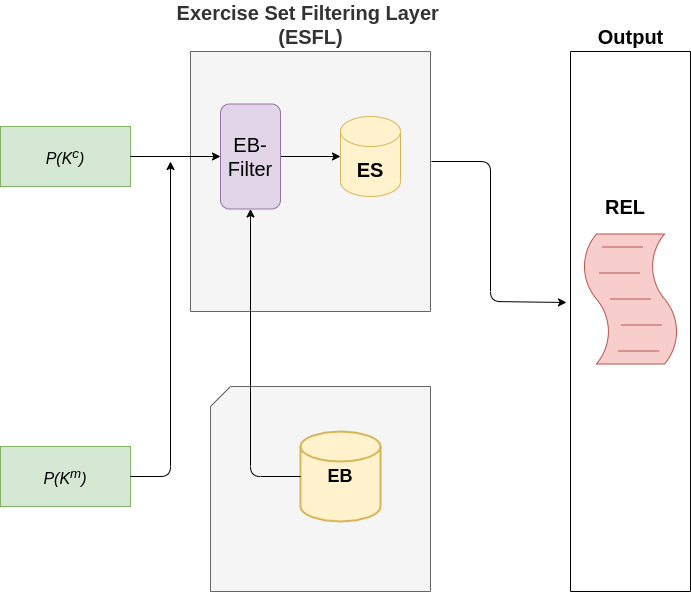
\includegraphics[scale=0.35]{charts/filterlayer.png}}
			\label{fig_motivation3}
			\caption{Exercise Set Filtering Layer (ESFL)}
		\end{figure}
	\end{frame}
	
	
	
	\section{Experimental} 	
	\begin{frame}{Experimental setup}
		\begin{itemize}
			\item Kaggle dataset is a subset of EdNet \footnote{\text{\color{blue} Youngduck Choi}, "EdNet: A Large-Scale Hierarchical Dataset in Education" \emph{\color{blue} In: arXiv:1912.03072.}}, published by Riiid Labs;
			\item Uses the LSTM network in the KCCP module to replace the Knowledge Graph which gives a probability distribution across all of the concepts contained in the course.
			\item For KCCP module use LSTM, we use F1-score, Accuracy, Precision and Recall for evaluation, while for KT module, use Accuracy and AUC metrics. With Exercises recommendation system in AL, we use 3 metrics: Accuracy, Novelty, and Diversity. \footnote{\text{\color{blue} }, "Exercises Recommendation System" \emph{\color{blue} In: \href{https://docs.google.com/document/d/1J11qjjtteFJDZnR8BaAcA\_ny6hT3wbt-ceO8G7hdKsk/}{Exercises Recommendation Literature Review}}}
		\end{itemize}
	\end{frame}
	
	\begin{frame}{KCCP module}
		\begin{figure}[htbp]
			\centerline{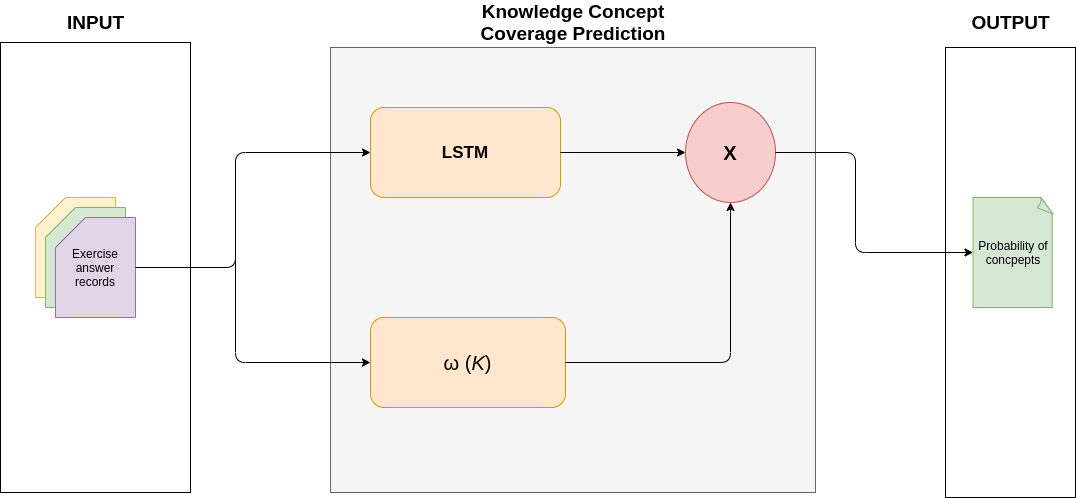
\includegraphics[scale=0.3]{charts/kccp.png}}
			\label{fig_motivation3}
			\caption{KCCP module use LSTM}
		\end{figure}
	\end{frame}
	
	\begin{frame}{Sub-modules results}
		Since the KG module is not available yet, we use a simple LSTM model instead. The input is the history learner interaction and the output is a probability distribution over concepts.
		
		\begin{table}
			\begin{tabular}{l | l | l | l | l}
				\hline
				Model & F1-Score & Accuracy & Precision & Recall\\
				\hline
				& & & & \\
				LSTM & 0.4561 & 0.4865 & 0.5253 & 0.4865\\ 
				& & & & \\
				\hline
			\end{tabular}
		\caption{KCCP module result.}
		\end{table}		
		
		\begin{table}
			\begin{tabular}{l | l | l }
				\hline
				Model & AUC & Accuracy \\
				\hline
				& & \\
				AKT-NR & 0.7754 & 0.7423\\ 
				 & & \\
				\hline
			\end{tabular}
		\caption{KT module result.}
		\end{table}
	\end{frame}
	
	\begin{frame}{System results}
		\begin{table}
			\begin{tabular}{l | l | l | l }
				\hline
				Model & Accuracy & Novelty & Diversity \\
				\hline
				& & & \\
				KCP-ER & 0.6548 & - & 0.3040 \\ 
				& & & \\
				\hline
			\end{tabular}
		\caption{Recommendation System result.}
		\end{table}
		
	\end{frame}
	
	
	
	\section{Next plan}
	\begin{frame}{Next plan}
		\begin{itemize}
			\item Improve model exercises recommendation includes: KCCP module, KT module, and algorithm to generate a Exercises subset with high diversity;
			\item Optimize the speed of system processing
			\item Implement and experiment ER model in Fschool dataset, analysis issues;
			\item Integrate into the production, running and waiting for the results !!!
		\end{itemize}
	\end{frame}
	
	
\end{document}
